\subsection{Implementation in Java}
\subsubsection{Berechnen der Sektoren}\label{BerechnenSektoren}
Die Größe des Bildes und in wie viele Teile dieses aufgeteilt werden soll ist bekannt. Dazu wird zum Beispiel die Breite des Bildes mit der horizontalen Anzahl an Sektoren geteilt. Ein Problem liegt darin, dass die Breite oder Höhe des Bildes nicht immer ein Vielfaches von den gewünschten Sektoren ist. Um das Problem zu lösen wird die Division mit Integers durchgeführt und der Rest gespeichert. Übergeblieben sind wie viele Spalten sich auf der X- und Y-Achse befinden und der Rest an Pixel. Im nächsten Schritt werden die Größen der Sektoren in Pixel berechnet. Es werden dazu zwei Integer Arrays für die X- und Y-Achse erschaffen. Jedes Element repräsentiert die Pixel Breite/Höhe seines Sektors. Standardmäßig besitzt jedes Element die Anzahl an Sektoren als Größe. Um den obigen berechneten Rest an Pixel zu verteilen, wird ein weiteres Array mit der Anzahl an Spalten als Länge aufsteigend nummeriert. Das Array wird anschließend von einer Methode gemischt. Eine abschließende Schleife wird mit der Anzahl des Restes wiederholt. Bei jedem Schritt wird ein dann zufälliger Wert aus dem Array als Index für das Array mit der Größe der Sektoren genutzt. Das nun zufällige Segment wird um 1 erhöht. Die berechneten Werte werden in einem \textit{splitObj} gespeichert. In diesem werden die Werte in unterschiedlichsten Arten wie z.B. Koordinaten gespeichert. 

Diese Koordinaten werden im nächsten Schritt benutzt, um ein zweidimensionales Array an \textit{BufferedImages} aus dem original Bild zu extrahieren. Dazu wird die \textit{getSubimage()} Methode der Klasse \textit{BufferedImage} verwendet.

\subsubsection{Berechnen der durchschnittlichen Farbe}
Das Berechnen der durchschnittlichen Farbe von Segmenten und Bildern ist die erste Funktion, welche Threads nutzt. Implementationen von mir, welche Threads benutzen, bestehen meistens aus zwei Klassen. Eine Klasse, welche die Threads erstellt und verwaltet und eine weitere, welche den Code zum berechnen der jeweiligen Anforderung beinhaltet. In diesem Falle das Berechnen der durchschnittlichen Farbe. Die Klasse \textit{computeAverageColor} besteht aus zwei Methoden. Eine zum berechnen der Segmente und eine weitere für die gewählten Bilder. Der einzige Unterschied der beiden Methoden ist eine Sicherheitsfunktion in der Methode der Bilder welche wartet, bis genügend RAM verfügbar ist, bevor es das Bild in den RAM läd. Dies ist wichtig, da mehrere Threads gleichzeitig die Bilder im RAM zum berechnen halten müssen. Je nach RAM Configuration und Bildergröße kann dies zu Komplikationen führen. Um zuverlässig die Größe des Bildes zu berechnen, kann nicht einfach die Dateigröße verwendet werden. Komprimierungsverfahren wie jpg und png kann die Dateigröße eines Bildes um das 10-fache verkleinern. Um die wirkliche Größe zu berechnen, müssen die Dimensionen und Farbtiefe verrechnet werden. Die verwendeten BufferedImages haben eine Farbtiefe von 4byte oder 32bit. Um die Dimensionen eines Bildes auszulesen, ohne das gesamte Bild in den Speicher laden zu müssen, wird die \textit{ImageIO} Klasse von java genutzt. Die \textit{ImageIO} Klasse bietet eine Methode, mit welcher alle \textit{ImageReader} eines Bildes erstellt werden. Ein \textit{ImageReader} benötigt lediglich die Metadaten eines Bildes, welche nur einen Bruchteil der Dateigröße entsprechen, um die Dimensionen des Bildes zu lesen. Jeder der Threads ruft die Methode \textit{getAverage()} der Klasse \textit{calculateAverage} auf. Die Methode verlangt ein \textit{BufferedImage} und ein enum \textit{calculateAverage.Method}, welches unterschiedliche Genauigkeitsstufen zum berechnen beinhaltet. Innerhalb der Methode \textit{getAverage()} wird erst mit Hilfe des enums ein Integer definiert, welches beschreibt wie stark die nachfolgenden for-Schleifen bei jedem Schritt erhöht werden soll. Weiterhin gibt es drei Long. Diese speichern den gesamten rot, blau und grün Wert des Bildes. Anschließend wird das Bild in der vorherigen definierten Schrittgröße durchgegangen und die rot, grün und blau Werte des Pixels gespeichert. Zum Schluss wird ein neues \textit{Color} Object mit den gesammelten Werten, geteilt durch die Anzahl der verwendeten Pixel, zurückgegeben.

\subsubsection{Erstellen einer Datenbank}
Dieser Schritt wird immer dann durchgeführt, wenn im Programm Bilder ausgewählt wurden, oder eine speicherbare Datenbank erstellt wird. Wenn Datenbanken ausgewählt wurden, wird die eventuell erstellte Datenbank diesen hinzugefügt. Die Klasse \textit{DatabaseObj} benötigt zwei Argumente. Eine Liste an Speicherorten der jeweiligen Bilder und ein Array an berechneten durchschnittlichen Farben. Innerhalb des \textit{DatabaseObj} werden die beiden Werte der Listen in \textit{fileAndColor} Objekten gespeichert. Wie der Name impliziert beinhalten die Objekte den Pfad des Bildes und den dazugehörigen Farbwert. Durch das Vorgehen kann ein BinarySort Algorithmus auf das neue Array angewendet werden. Dazu hat die \textit{fileAndColor} Klasse das \textit{Comparable} interface implementiert. Für spätere Verwendung gibt es in den Objekten auch noch einen Zähler, welcher speichert, wie häufig das Bild in der Berechnung verwendet wurde. Alle Variablen der Klasse \textit{fileAndColor} sind durch getter- setter-Methoden aufzurufen. Diese haben die Besonderheit, dass sie das \textit{synchronized} Schlüsselwort besitzen (siehe Abschnitt \ref{Threadsicherheit}).
\bigskip
\newline
Besonders werde ich auf die Methode \textit{compareTo()}, des Interfaces Comparable eingehen. In der Methode werden zwei Farben verglichen. Die Schwierigkeit liegt darin ein Ergebnis zu bestimmen, wenn vier Werte verglichen werden müssen, der alpha-Wert, rot-Wert, grün-Wert und blau-Wert. Um ein einfachen und zuverlässigen Vergleich zu machen, nutze ich die Methode \textit{getRGB()} der \textit{Color} Klasse. Interessant ist jedoch, was diese Methode macht. In der Klasse \textit{Color} werden alle vier Werte in einem einzigen Integer gespeichert. Das liegt an der Genauigkeit womit Farben gemischt werden. Jeder Wert befindet sich in einem Bereich von 0 bis 255. Dies entspricht genau einem Byte. Ein Integer wiederum besteht aus vier Bytes. Die vier Farbwerte werden sozusagen in die vier Bytes des Integers eingesetzt. In der Reihenfolge ``ARGB''.\\
\begin{figure}[h]
    \centering
    \begin{tabular}{c | c | c | c || c}
        alpha(255) & rot(224) & grün(64) & blau(16) & \tikz \definecolor{dkOrange}{rgb} {0.88,0.25,0.06} \fill [dkOrange] (0, 0) rectangle (10pt, 10pt); \\
        \hline
        11111111 & 11100000 & 01000000 & 00010000 & -2080752
    \end{tabular}
\end{figure}
\\Durch dieses Vorgehen wird aus vier Werten ein zuverlässiger Wert erstellt, welcher zum sortieren geeignet ist.

\newpage

\subsubsection{Berechnen der besten Bilder}
Das Berechnen der besten Bilder für die jeweiligen Sektoren wird in der Klasse \textit{compareColor} mit der Methode \textit{compare()} ausgeführt. Die Methode gibt ein zweidimensionales \textit{File}-Array zurück. Dies steht dabei für die einzelnen Sektoren. Innerhalb der Methode wird für jeden Sektor ein \textit{Runnable} erstellt. (siehe Abschnitt \ref{ThreadsInJava}). Da es ein Limit für die Verwendung der Bilder gibt, sollen diese gleichmäßig verteilt werden. Um einen solchen Effekt zu erhalten wird eine Liste an \textit{Runnables} erstellt und gemischt.

\begin{figure}[h]
    \centering
    \subfloat[\centering ohne Mischung]{
        \includegraphics[height=5cm]{images/BadExample_Lines.pdf}
    }
    \subfloat[\centering mit Mischung]{
        \includegraphics[height=5cm]{images/GodExample_NoLines.pdf}
    }
    \caption[Beste Bilder]{Unterschied zwischen mischen und nicht mischen}
\end{figure}

\begin{sloppypar}
Jeder \textit{Runnable} sucht demnach nach dem besten Bild, welches noch verfügbar ist. Aus jeder Datenbank wird mithilfe einer binären Suche das beste Bild bestimmt. Diese werden untereinander verglichen und das finale Bild bestimmt. Die binäre Suche wird mithilfe der Java Methode \textit{Arrays.binarySearch} realisiert werden. Sie findet nicht nur den exakten Wert, sondern auch einen Index, wo er sich befinden könnte. Um das Verwendungslimit eines Bildes nicht zu überschreiten wird, von dem Index als Mitte, immer weiter nach links und rechts gegangen. Die beiden Werte, werden auf Farbnähe zum mittigen Wert überprüft. Der Nähere wird dementsprechend auserwählt. Durch die Nutzung der \textit{fileAndColor} Klasse ist der Speicherort des Bildes bekannt.
\end{sloppypar}

\newpage

\subsubsection{Skalieren der Bilder}
Das Skalieren der Bilder ist in drei Schritte einzuteilen. Das Management der Bilder, berechnen der Zielgröße und das Skalieren an sich. Ich werde auf jeden Bereich individuell eingehen.

\paragraph{Management}\mbox{}\\
Da ein Bild mehrfach ausgewählt werden kann, ist es wichtig ein Management System zu haben, welches verhindert, dass das selbe Bild nicht häufiger als nötig skaliert wird. Das Skalieren ist der zeitaufwendigste Prozess, daher sollte dieser minimiert werden. Jedes Bild wird in vier unterschiedlichen Größen verwendet werden. Die Größen entstehen aus dem in Abschnitt \ref{BerechnenSektoren} beschriebenen Vorgehen. Werden die Bilder nur in einer einheitlichen Größe skaliert entstehen schwarze Linien im Bild.

\begin{figure}[h]
    \centering
    \subfloat[\centering ohne mehrfach Skalierung]{
        \includegraphics[height=5cm]{images/BadExample_BlackLines.pdf}
    }
    \subfloat[\centering mit mehrfach Skalierung]{
        \includegraphics[height=5cm]{images/GodExample_NoBlackLines.pdf}
    }
    \caption[Schwarze Linien]{vierfache Skalierung der Bilder}
\end{figure}

Beim Managen wird demnach überprüft, ob ein bestimmtes Bild schon in der jeweiligen Größe vorhanden ist. Dazu wird eine Instanz der Klasse \textit{ScaledImages} erzeugt. Diese Instanz fungiert als gemeinsamer Speicherort aller skalierten Bilder. Die Klasse hat ein zweidimensionales Array des Types \textit{ImageWithName} und eine Methode \textit{exists()}. Die Methode \textit{exists()} sucht mithilfe von dem Pfad des Bildes und den gewünschten Dimensionen in dem Array nach bereits skalierten Bildern. In dem Fall, dass etwas gefunden wird, werden die Koordinaten des gefunden Bildes zurückgegeben. Im Falle eines Treffers wird eine Referenz auf das Bild gespeichert, anstelle es zu skalieren.
\medskip
\newline
Ein Problem beinhaltet das System jedoch noch. Es könnte zu der Situation kommen, dass mehrere Threads gleichzeitig mit dem gleichem Bildauftrag gestartet werden. Anfangs überprüft jeder Thread, ob sie arbeiten dürfen, oder das gewünschte Bild noch nicht existiert. Alle Threads werden davon ausgehen, dass sie arbeiten dürfen. Denn das Skalieren des Bildes und Speichern dessen länger dauert als einen neuen Thread zu starten. Doch dadurch werden nicht nur Ressourcen unnütz verbraucht, sondern auch Fehler in der Bilddatei können durch gleichzeitiges zugreifen auf eine Datei entstehen.

\begin{figure}[h]
    \centering
    \begin{minipage}{89mm}
        \fontsize{10pt}{11pt}\selectfont
        \def\svgwidth{8cm}
        \input{images/Manager_Threads.pdf_tex}
    \end{minipage}
    \begin{minipage}{1\textwidth-91mm}
        1. Überprüfen, ob die Bilder schon vorhanden sind.\\
        2. Schreiben des Bildes in das Array.
    \end{minipage}
    \caption[Thread und Manager]{Threads mit Manager}
\end{figure}

Um ein solches Verhalten zu verhindern, versucht ein Thread ein Bild zu reservieren, wenn es laut Manager frei ist. Ein reserviertes Bild wird als bereits existierendes gewertet. Das Referenz System funktioniert weiterhin, da nur auf den Index gezeigt wird und nicht auf dessen Inhalt. Die für gewöhnlich lineare Array Struktur wird durch rasantes steigen des Speicherverbrauchs einzelner Objekte nicht beeinflusst. Das liegt unter anderem an dem \textit{GarbageCollector} von Java, welcher auch im Stande ist Arrays aus ihrem sonst linearem Besetzen eines Speicherblockes im Arbeitsspeicher aufzuteilen. Es kann dadurch  größer werdenden Objekten Platz geschaffen werden. Interne Referenzen des Arrays werden überschrieben, um zu dem verschobenem Objekt zu zeigen.

\newpage

\paragraph{Berechnen der Zielgröße}\mbox{}\\
Das Ziel ist, die Bilder so gut wie möglich zu verwerten. Dazu müssen unterschiedliche Kriterien erfüllt werden. Erstens sollte das Bild nicht verzogen werden, zweitens sollte immer der größtmögliche Bereich eines Bildes verwendet werden.

\begin{figure}[h]
    \centering
    \fontsize{12pt}{12pt}\selectfont% or whatever fontsize you like
    \def\svgwidth{12cm}
    \input{images/BerechnenZielgröße.pdf_tex}
    \caption[Berechnen Zielgröße]{Berechnen Zielgröße}
\end{figure}

Um das erreichen zu können, wird das Bild erst auf die Größe des gewünschten Sektors skaliert. Anschließend werden die Ränder abgeschnitten. Beim Skalieren wird versucht die x-Achse des Bildes der y-Achse des Sektors anzupassen. Damit kann sichergestellt werden, dass das Bild sein Verhältnis beibehält. Wie in der oberen Grafik zu erkennen ist, wird ein vertikal ausgerichtetes Bild in einen horizontalen Sektor eingesetzt. Dazu wurde die x-Achse des Bildes auf die des Sektors skaliert. Die Formel zum Berechnen der y-Achse ist wie folgt.
\begin{align}
    y_\mathnormal{Bild\,neu}=y_\mathnormal{Bild\,alt} \cdot \frac{x_\mathnormal{sek.}}{x_\mathnormal{Bild\,alt}}
\end{align}    
Wenn die neu berechnete y-Achse kleiner ist als die des Sektors, wird das obige Vorgehen umgekehrt mit der x-Achse gemacht. Der letzte Schritt ist ein Abschnitt mittig aus dem skaliertem Bild mit den Abmaßen des Sektors zu schneiden.

\newpage

\paragraph{Skalieren des Bildes}\mbox{}\\
Einleitend muss ich zu diesem Abschnitt sagen, dass ich die folgenden Methoden nicht selber implementiert habe. Ich nutzte dazu die imgskalr library von Riyad Kalla, welche auf der bilinearen und bikubischen Interpolation von Javas \textit{Graphics2D} beruht.\cite{Scalr:Kalla} Im folgenden werde ich die Bilineare Interpolation erklären. Auf die bikubischen Interpolation werde ich nur kurz eingehen.
\medskip
\newline
Bei dem Hochskalieren von Bildern stößt man auf das Problem, dass Farbwerte erfunden werden müssen. Andere Algorithmen erfinden keine neuen Farben und sind gut für Pixel Bilder geeignet (nearest neighbour). Für Landschaftsbilder würde dies lediglich ein verpixeltes Bild in einer größeren Auflösung ergeben. Um neue Farbwerte zu berechnen, werden diese bei der bilinearen Interpolation linear zwischen den Pixeln ermittelt.

\begin{figure}[h]
    \centering
    \subfloat[\centering Bilinear Start]{
        \input{images/bilinearInterpolation.tex}
    }
    \subfloat[\centering Bilinear Ende]{
        \tdplotsetmaincoords{50}{-15}
    \begin{tikzpicture}[tdplot_main_coords, scale = 1]
        \filldraw[draw = black, fill = blue, opacity = 0.2](0,0,0) -- (3,0,0) -- (3, 3, 0) -- (0, 3, 0);

        \def \xy{{  {2, 1, 0.5, 1}, 
                    {4, 1, 2, 3}, 
                    {3, 2, 4, 1}, 
                    {0.5, 3, 5, 4}}}

        \foreach \x in {0,...,3}{
            \foreach \y in {0,...,3}{
                \draw[fill = black](0,0,0) circle (2pt);
                \pgfmathsetmacro\asInt{int(\xy[\x][\y])}
                \pgfmathsetmacro\r{(\asInt+1)/2}
                \draw[black](\x, 0, 0) -- (\x,3,0);
                \draw[black](0,\y,0) -- (3,\y,0);
                %bottom
                \filldraw[draw = black, fill = red, opacity = 0.2](\x,\y,0) -- (\x+1,\y,0) -- (\x+1,\y+1,0) -- (\x,\y+1,0);
                %top
                \filldraw[draw = black, fill = red, opacity = 0.5](\x,\y,\r) -- (\x+1,\y,\r) -- (\x+1,\y+1,\r) -- (\x,\y+1,\r);
                %front
                \filldraw[draw = black, fill = red, opacity = 0.2](\x,\y,0) -- (\x+1,\y,0) -- (\x+1,\y,\r) -- (\x,\y,\r);
                %back
                \filldraw[draw = black, fill = red, opacity = 0.2](\x,\y+1,0) -- (\x+1,\y+1,0) -- (\x+1,\y+1,\r) -- (\x,\y+1,\r);
                %rigth
                \filldraw[draw = black, fill = red, opacity = 0.3](\x+1,\y,0) -- (\x+1,\y+1,0) -- (\x+1,\y+1,\r) -- (\x+1,\y,\r);
                %left
                \filldraw[draw = black, fill = red, opacity = 0.4](\x,\y,0) -- (\x,\y+1,0) -- (\x,\y+1,\r) -- (\x,\y,\r);
            }
        }
        \foreach \x in {0,...,2}{
            \foreach \y in {0,...,2}{
                \pgfmathsetmacro\asInt{int(\xy[\y][\x])}
                \pgfmathsetmacro\r{(\asInt+1)/2}
                
                \pgfmathsetmacro\nextx{\x==2 ? \x+0.5 : \x+1.5}
                \pgfmathsetmacro\nexty{\y==2 ? \y+0.5 : \y+1.5}

                \pgfmathsetmacro\nextXAsInt{int(\xy[int(\y)][int(\nextx)])}
                \pgfmathsetmacro\nextXr{(\nextXAsInt+1)/2}
                \pgfmathsetmacro\nextYAsInt{int(\xy[int(\nexty)][int(\x)])}
                \pgfmathsetmacro\nextYr{(\nextYAsInt+1)/2}
                \pgfmathsetmacro\nextXYAsInt{int(\xy[int(\nexty)][int(\nextx)])}
                \pgfmathsetmacro\nextXYr{(\nextXYAsInt+1)/2}

                \draw[thick, blue, -](\x+0.5,\y+0.5,0) -- (\x+0.5,\y+0.5,\r);
                \draw[fill = blue](\x+0.5,\y+0.5,\r) circle (2pt);
                \draw[thick, green, -](\x+0.5,\y+0.5,\r) -- (\nextx,\y+0.5,\nextXr);
                \draw[thick, green, -](\x+0.5,\y+0.5,\r) -- (\x+0.5,\nexty,\nextYr);
                
                \ifnum\x<2
                \ifnum\y<2
                    \pgfmathsetmacro\stepXY{1/2}
                    \pgfmathsetmacro\stepXXR{(\nextXr-\r)/2}
                    \pgfmathsetmacro\stepYYR{(\nextYr-\r)/2}
                    \pgfmathsetmacro\stepXYR{(\nextXYr-\nextYr)/2}
                    \pgfmathsetmacro\stepYXR{(\nextXYr-\nextXr)/2}
                    \foreach \xx in {0,...,0}{
                        \foreach \yy in {0,...,0}{
                            \pgfmathsetmacro\newX{\stepXY*(\xx+1)}
                            \pgfmathsetmacro\newY{\stepXY*(\yy+1)}
                            \pgfmathsetmacro\newXR{\r+\stepXXR*(\xx+1)}
                            \pgfmathsetmacro\newYR{\r+\stepYYR*(\yy+1)}
                            
                            \pgfmathsetmacro\nextYR{\nextYr+\stepXYR*(\xx+1)}
                            \pgfmathsetmacro\nextXR{\nextXr+\stepYXR*(\yy+1)}

                            \draw[thick, orange, -](\x+0.5+\newX,\y+0.5,\newXR) -- (\x+0.5+\newX,\y+1.5,\nextYR);
                            \draw[thick, orange, -](\x+0.5,\y+0.5+\newY,\newYR) -- (\x+1.5,\y+0.5+\newY,\nextXR);
                        }
                    }
                \fi
                \fi
            }
        }
    \end{tikzpicture}
    }
    \caption[Bilinear]{Bilineare Interpolation}
\end{figure}

Die unterschiedlichen Höhen in der Grafik, repräsentieren die unterschiedlichen Farbwerte der Pixel. Das 3x3 Bild wird um den Faktor 3 skaliert. Zuerst wird ein Netz zwischen den einzelnen Werten gespannt. Die neuen Farbwerte entstehen an den Schnittpunkten des Netzes. Der Farbwert lässt sich somit mit den folgenden Gleichungen berechnen.\cite[Ab 4:44]{Bilinear:Pound}
\begin{flalign}
    F_\mathnormal{neuX}=(F_\mathnormal{1\,0}-F_\mathnormal{0\,0})\cdot\frac{n_x}{S_\mathnormal{fak.}} \label{eq:WNeuX}\\
    F_\mathnormal{neuY}=(F_\mathnormal{1\,1}-F_\mathnormal{0\,1})\cdot\frac{n_y}{S_\mathnormal{fak.}} \label{eq:WNeuY}\\
    F_\mathnormal{neu}=F_\mathnormal{0\,0}+(F_\mathnormal{neuX})+(F_\mathnormal{neuY}-F_\mathnormal{neuX})\cdot\frac{n_y}{S_\mathnormal{fak.}} \label{eq:WNeu}
\end{flalign}
In den Gleichungen \ref{eq:WNeuX} und \ref{eq:WNeuY} werden die Start- und End-Punkte einer Netzlinie berechnet. $n_x$ und $n_y$ sind Zähler, welche die gewünschte Position in dem Teilnetz angeben. Das Maximum der beiden ist $S_\mathnormal{fak.}+1$. $S_\mathnormal{fak.}$ ist dabei der Faktor, um wie viel das Bild skaliert werden soll.
\medskip
\newline
Der Unterschied zischen bilinearer und bikubischen Interpolation ist, dass bei der bilinearen Interpolation lediglich zwei Linien aus jeweils zwei Punkte benutzt werden. Bei der bikubischen Interpolation werden vier kubische Spline Funktionen aus jeweils vier Punkten benutzt. Der Vorteil der bikubischen Interpolation ist, dass das resultierende Bild einen höheren Kontrast bekommt. Auch können komplexere Formen besser berücksichtigt werden.\cite[Seite 37]{Bicubic:Rowe}

\begin{figure}[h]
    \centering
    \subfloat[\centering Bilinear]{
        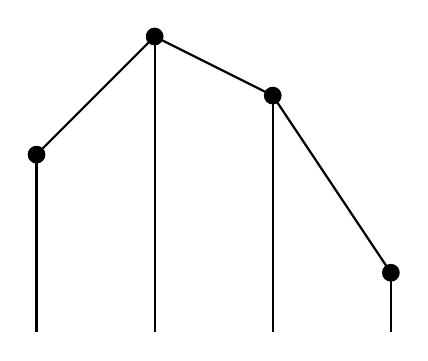
\begin{tikzpicture}[scale = 1.5]
    \def \valY{{2, 4, 3, 0.5}}

    \foreach \x in {0,...,3}{
        \pgfmathsetmacro\asInt{int(\valY[\x])}
        \pgfmathsetmacro\r{(\asInt+1)/2}
        \draw[thick, black, -](\x,0) -- (\x,\r);
        \draw[fill = black](\x,\r) circle (2pt);
        
        \pgfmathsetmacro\nextx{\x==3 ? \x : \x+1}
        \pgfmathsetmacro\nextAsInt{int(\valY[\nextx])}
        \pgfmathsetmacro\nextR{(\nextAsInt+1)/2}
        \draw[thick, black, -](\x,\r) -- (\nextx,\nextR);
    }
\end{tikzpicture}
    }
    \subfloat[\centering Bikubisch \protect\footnotemark]{
        %Berechnet mit https://tools.timodenk.com/cubic-spline-interpolation

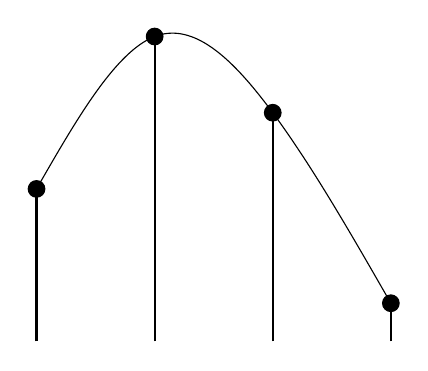
\begin{tikzpicture}[scale = 1.5]
    
        \pgfmathsetmacro\rEins{(+-0.7*0^3+1.32e-62*0^2+2.7*0^1+2*0^0)/1.55}
        \draw[thick, black, -](0,0) -- (0,\rEins);
        \draw[fill = black](0,\rEins) circle (2pt);

        \pgfmathsetmacro\rZwei{(+-0.7*1^3+1.32e-62*1^2+2.7*1^1+2*1^0)/1.55}
        \draw[thick, black, -](1,0) -- (1,\rZwei);
        \draw[fill = black](1,\rZwei) circle (2pt);

        \pgfmathsetmacro\rDrei{(+0.5*2^3+-3.6*2^2+6.3*2^1+0.8*2^0)/1.55}
        \draw[thick, black, -](2,0) -- (2,\rDrei);
        \draw[fill = black](2,\rDrei) circle (2pt);

        \pgfmathsetmacro\rVier{(+0.2*3^3+-1.8*3^2+2.7*3^1+3.2*3^0)/1.55}
        \draw[thick, black, -](3,0) -- (3,\rVier);
        \draw[fill = black](3,\rVier) circle (2pt);


    \draw[domain=0:1, smooth, variable=\x, black] plot ({\x}, {(+-0.7*\x^3+1.32e-62*\x^2+2.7*\x^1+2*\x^0)/1.55});
    \draw[domain=1:2, smooth, variable=\x, black] plot ({\x}, {(+0.5*\x^3+-3.6*\x^2+6.3*\x^1+0.8*\x^0)/1.55});
    \draw[domain=2:3, smooth, variable=\x, black] plot ({\x}, {(+0.2*\x^3+-1.8*\x^2+2.7*\x^1+3.2*\x^0)/1.55});
\end{tikzpicture}
    }
    \caption[BilinearBikubisch]{Vergleich Bilinear und Bikubisch}
\end{figure}
\footnotetext{Funktion mit \url{https://tools.timodenk.com/cubic-spline-interpolation} erstellt}

\medskip
Um die beste Qualität bei dem runterskalieren zu erhalten, wird das Bild häufiger skaliert. Dies verwaltet die imgskalr library. Das Bild wird wiederholt um $\frac{1}{7}$ seiner Breite und Höhe verkleinert. Der Wert wurde nicht mathematisch berechnet, sondern wurde durch testen herausgefunden.\cite[Scalr.java Zeile 2221]{Scalr:Kalla}

\begin{figure}[h]
    \centering
    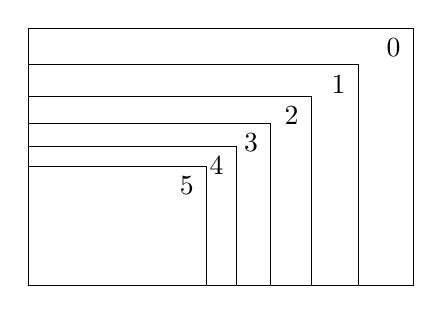
\begin{tikzpicture}[scale = 0.1]
    \def \xy {{{4890,3263},
               {4192,2797},
               {3594,2398},
               {3081,2056},
               {2641,1763},
               {2264,1512}}}

    \foreach \x in {0,...,5}{
        \pgfmathsetmacro\width{int(\xy[\x][0])/100}
        \pgfmathsetmacro\height{int(\xy[\x][1])/100}
        \draw[black](0,0)--(\width,0)--(\width,\height)--(0,\height)--(0,0);
        \node[] at (\width-2.5,\height-2.5) (a) {\x};
    }

\end{tikzpicture}
    \caption[Inkrementell]{Inkrementelles Skalieren}
\end{figure}